\documentclass{beamer}
\usepackage[utf8]{inputenc}
\usepackage{lipsum}
\usepackage{multirow}
\usepackage{graphicx}
\usepackage{tabularx}
\usepackage{booktabs}
\usepackage{hyperref}
\usepackage[style=authortitle,backend=bibtex]{biblatex}
\addbibresource{ref.bib}





\graphicspath{ {./images/} }
\usepackage{cellspace}
\usepackage{tikz}

\setlength\cellspacetoplimit{5pt}
\setlength\cellspacebottomlimit{5pt}
%\setbeameroption{show notes}
\usetheme{Madrid}
\usecolortheme{default}
\newcommand{\credit}[1]{\par\hfill \footnotesize Data Source:~\itshape#1}


%Information to be included in the title page:
\title{Analysis of Electricity Consumption in India}
\author{Group- WATTSUP}
%\institute{IIM}

\date{November 2021}

\begin{document}
\AtBeginSection[]{
  \begin{frame}{Outline}
  \small \tableofcontents[currentsection, hideothersubsections]
  \end{frame} 
}
\begin{frame}[noframenumbering, plain]
\centering

\includegraphics[width=3cm]{images/logo.png}

\includegraphics[width=3cm]{images/logo.png}
\titlepage
\end{frame}
%\frame{\titlepage}
\begin{frame}
\frametitle{Table of Contents}
\tableofcontents
\end{frame}

\section{Objectives}
\begin{frame}{What we set out to do}
\centering
\includegraphics[scale=.75]{images/Objective.png}
\end{frame}


\begin{frame}{What we will attempt to do}
\begin{block}{Time series Analysis}
    Undertake time series analysis of peak electricity consumption and model the time series      
\end{block}
\begin{block}{Predict Net Zero emission goals}
    \begin{itemize}
        \item COP26
        \begin{itemize}
            \item Reduce Fossil fuel dependence to 50%
            \item Net Zero carbon emission by 2070
        \end{itemize}
        Analyse if we are on track to achieve net zero emission by 2070
    \end{itemize}

\end{block}

\end{frame}

\section{Time Series}
\subsection{Data Review}

\begin{frame}{Data Quality Characteristics}
\centering
 
 \begin{table}
     \centering
     
     \begin{tabular}{lll}
        Characteristic & Description & Remarks\\
        \toprule
        
         Source & Niti Ayog Website & https://iced.niti.gov.in/\\ \hline
          Period & 20 Apr 17 to  06 Nov 23 & \\  \hline
          Periodicity & Daily & \\  \hline
          Observation & Daily Peak Demand  &  in MW \\ \hline
          \# of Observations & 2390  & \\  \hline
          Range & 115232 to 239978  &  in MW \\ 
          \bottomrule
     \end{tabular}
     \caption{Data Characteristics}
     \label{tab:my_label}
 \end{table}

\end{frame}

\begin{frame}{Plot of Data}
\centering
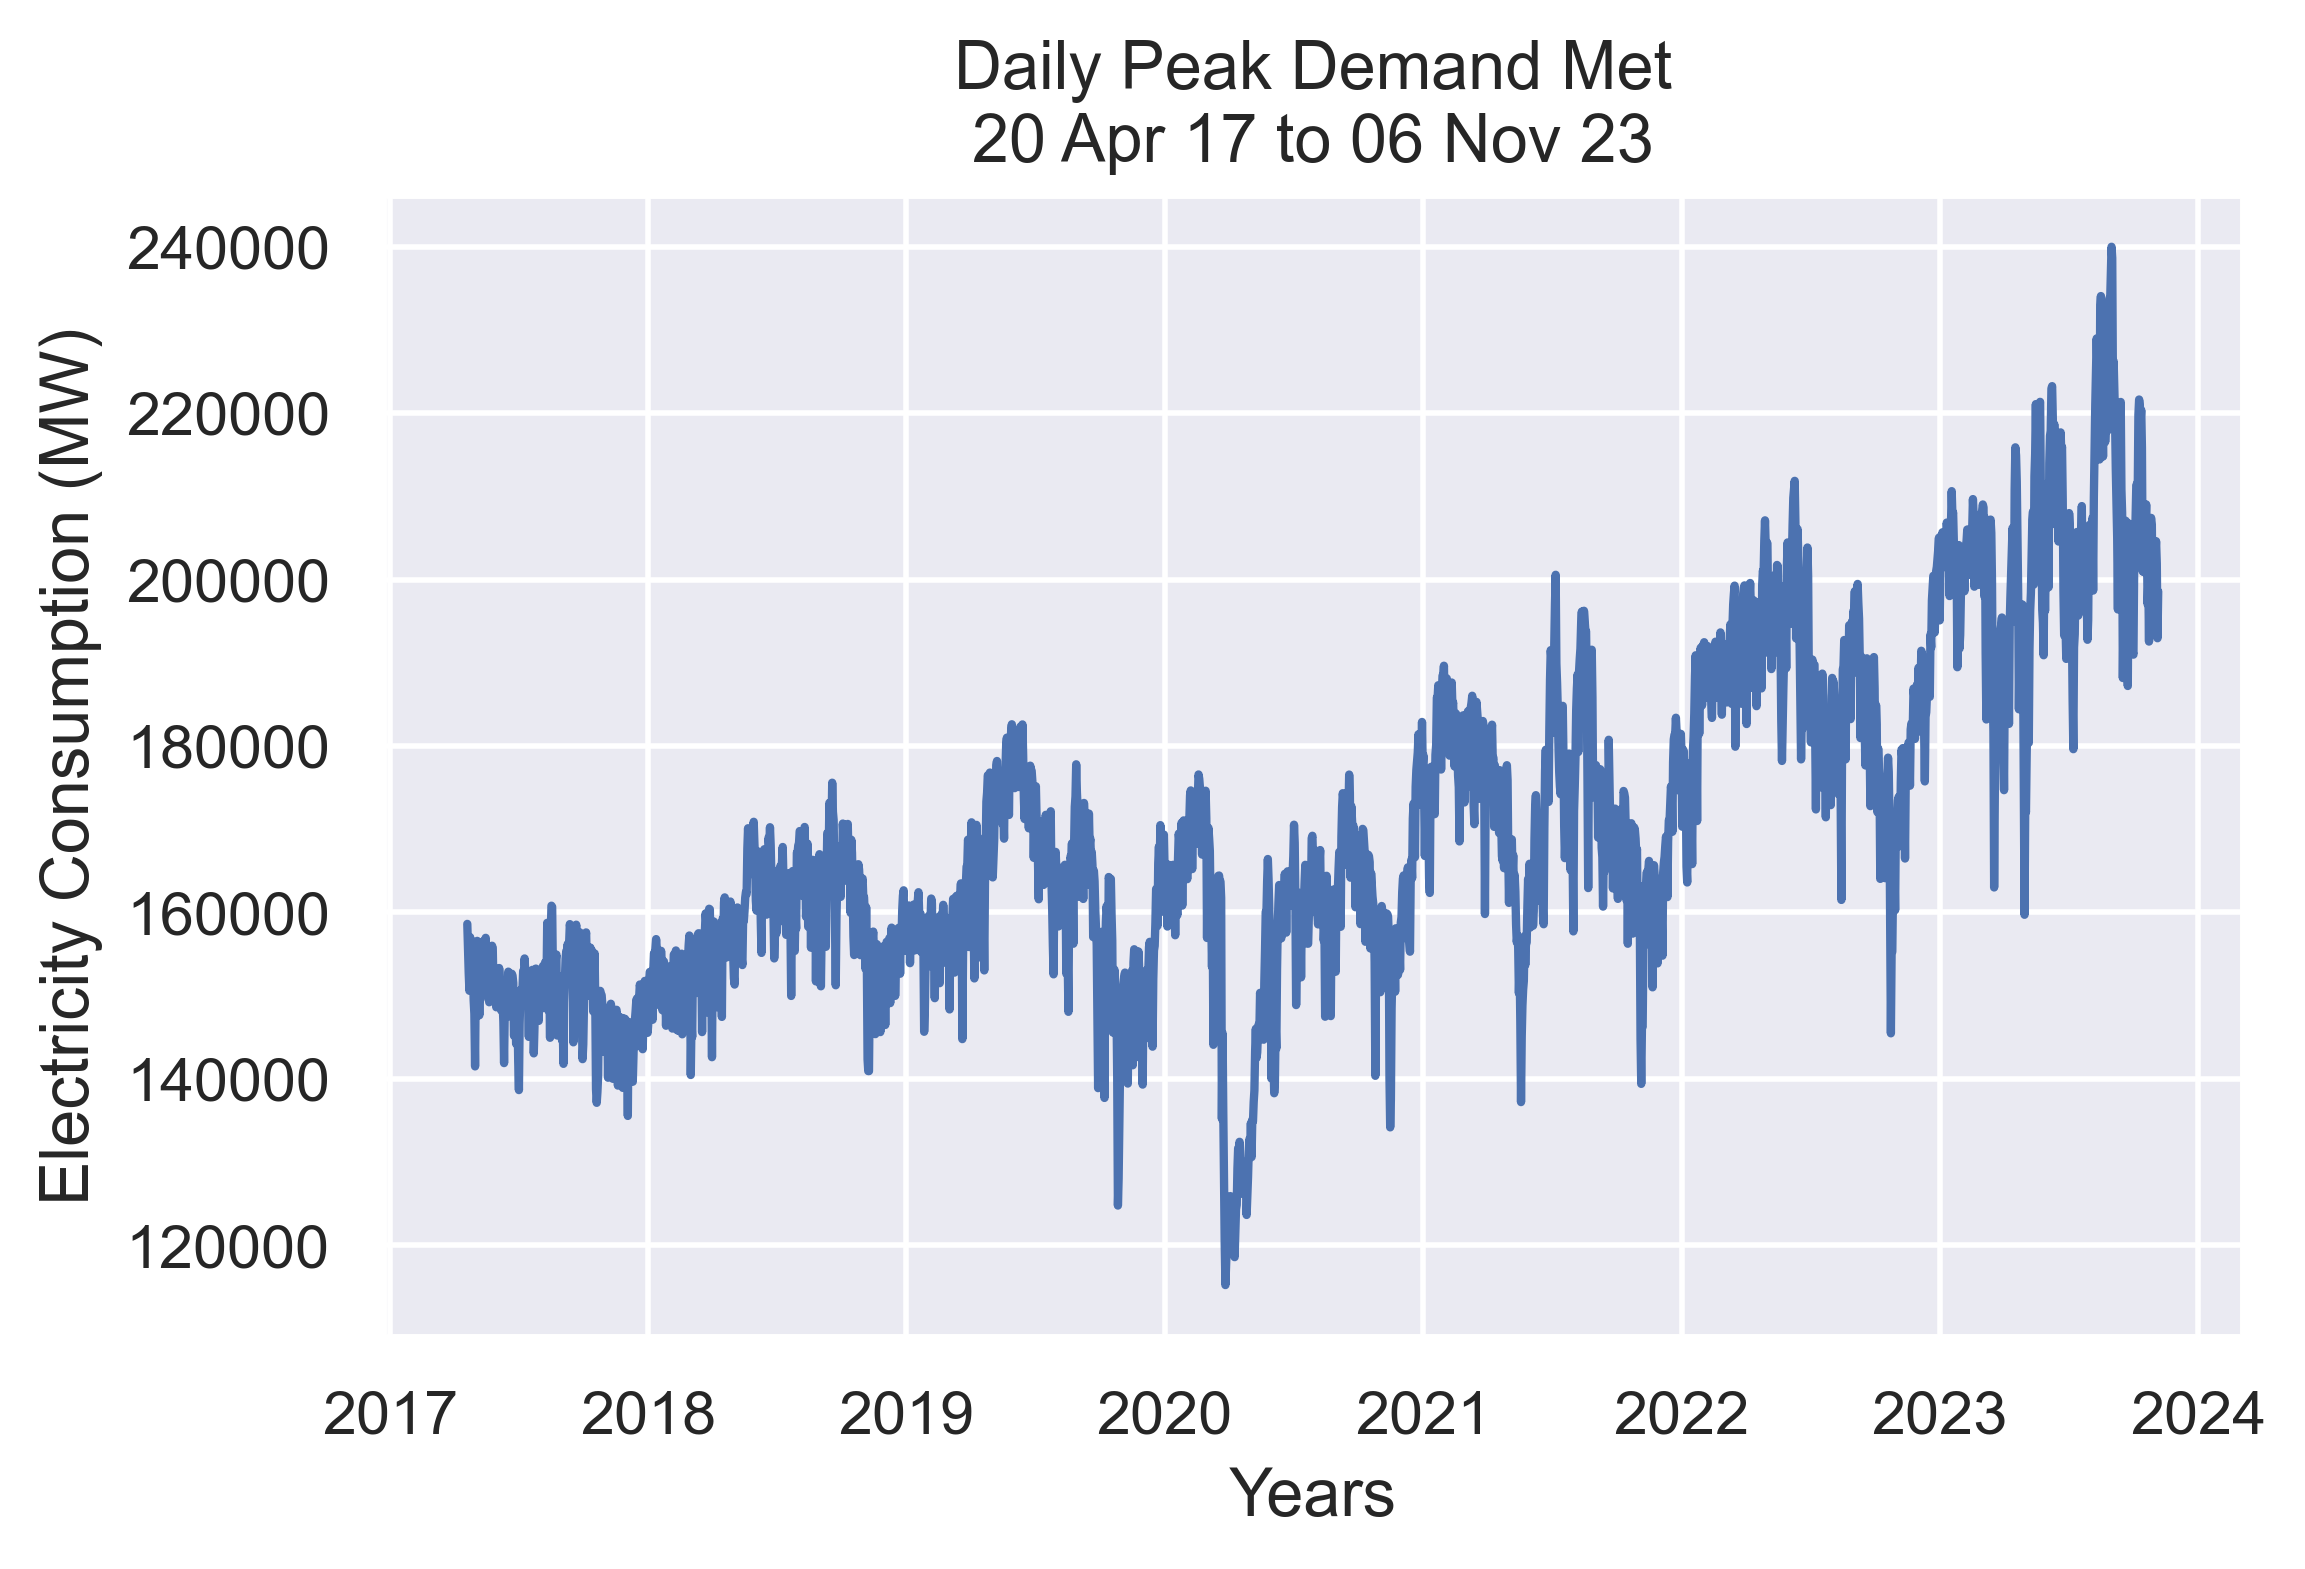
\includegraphics[scale=.75]{images/Daily Peak.png}
\credit{https://iced.niti.gov.in/}
\end{frame}


\begin{frame}{Plot of Data}
\centering
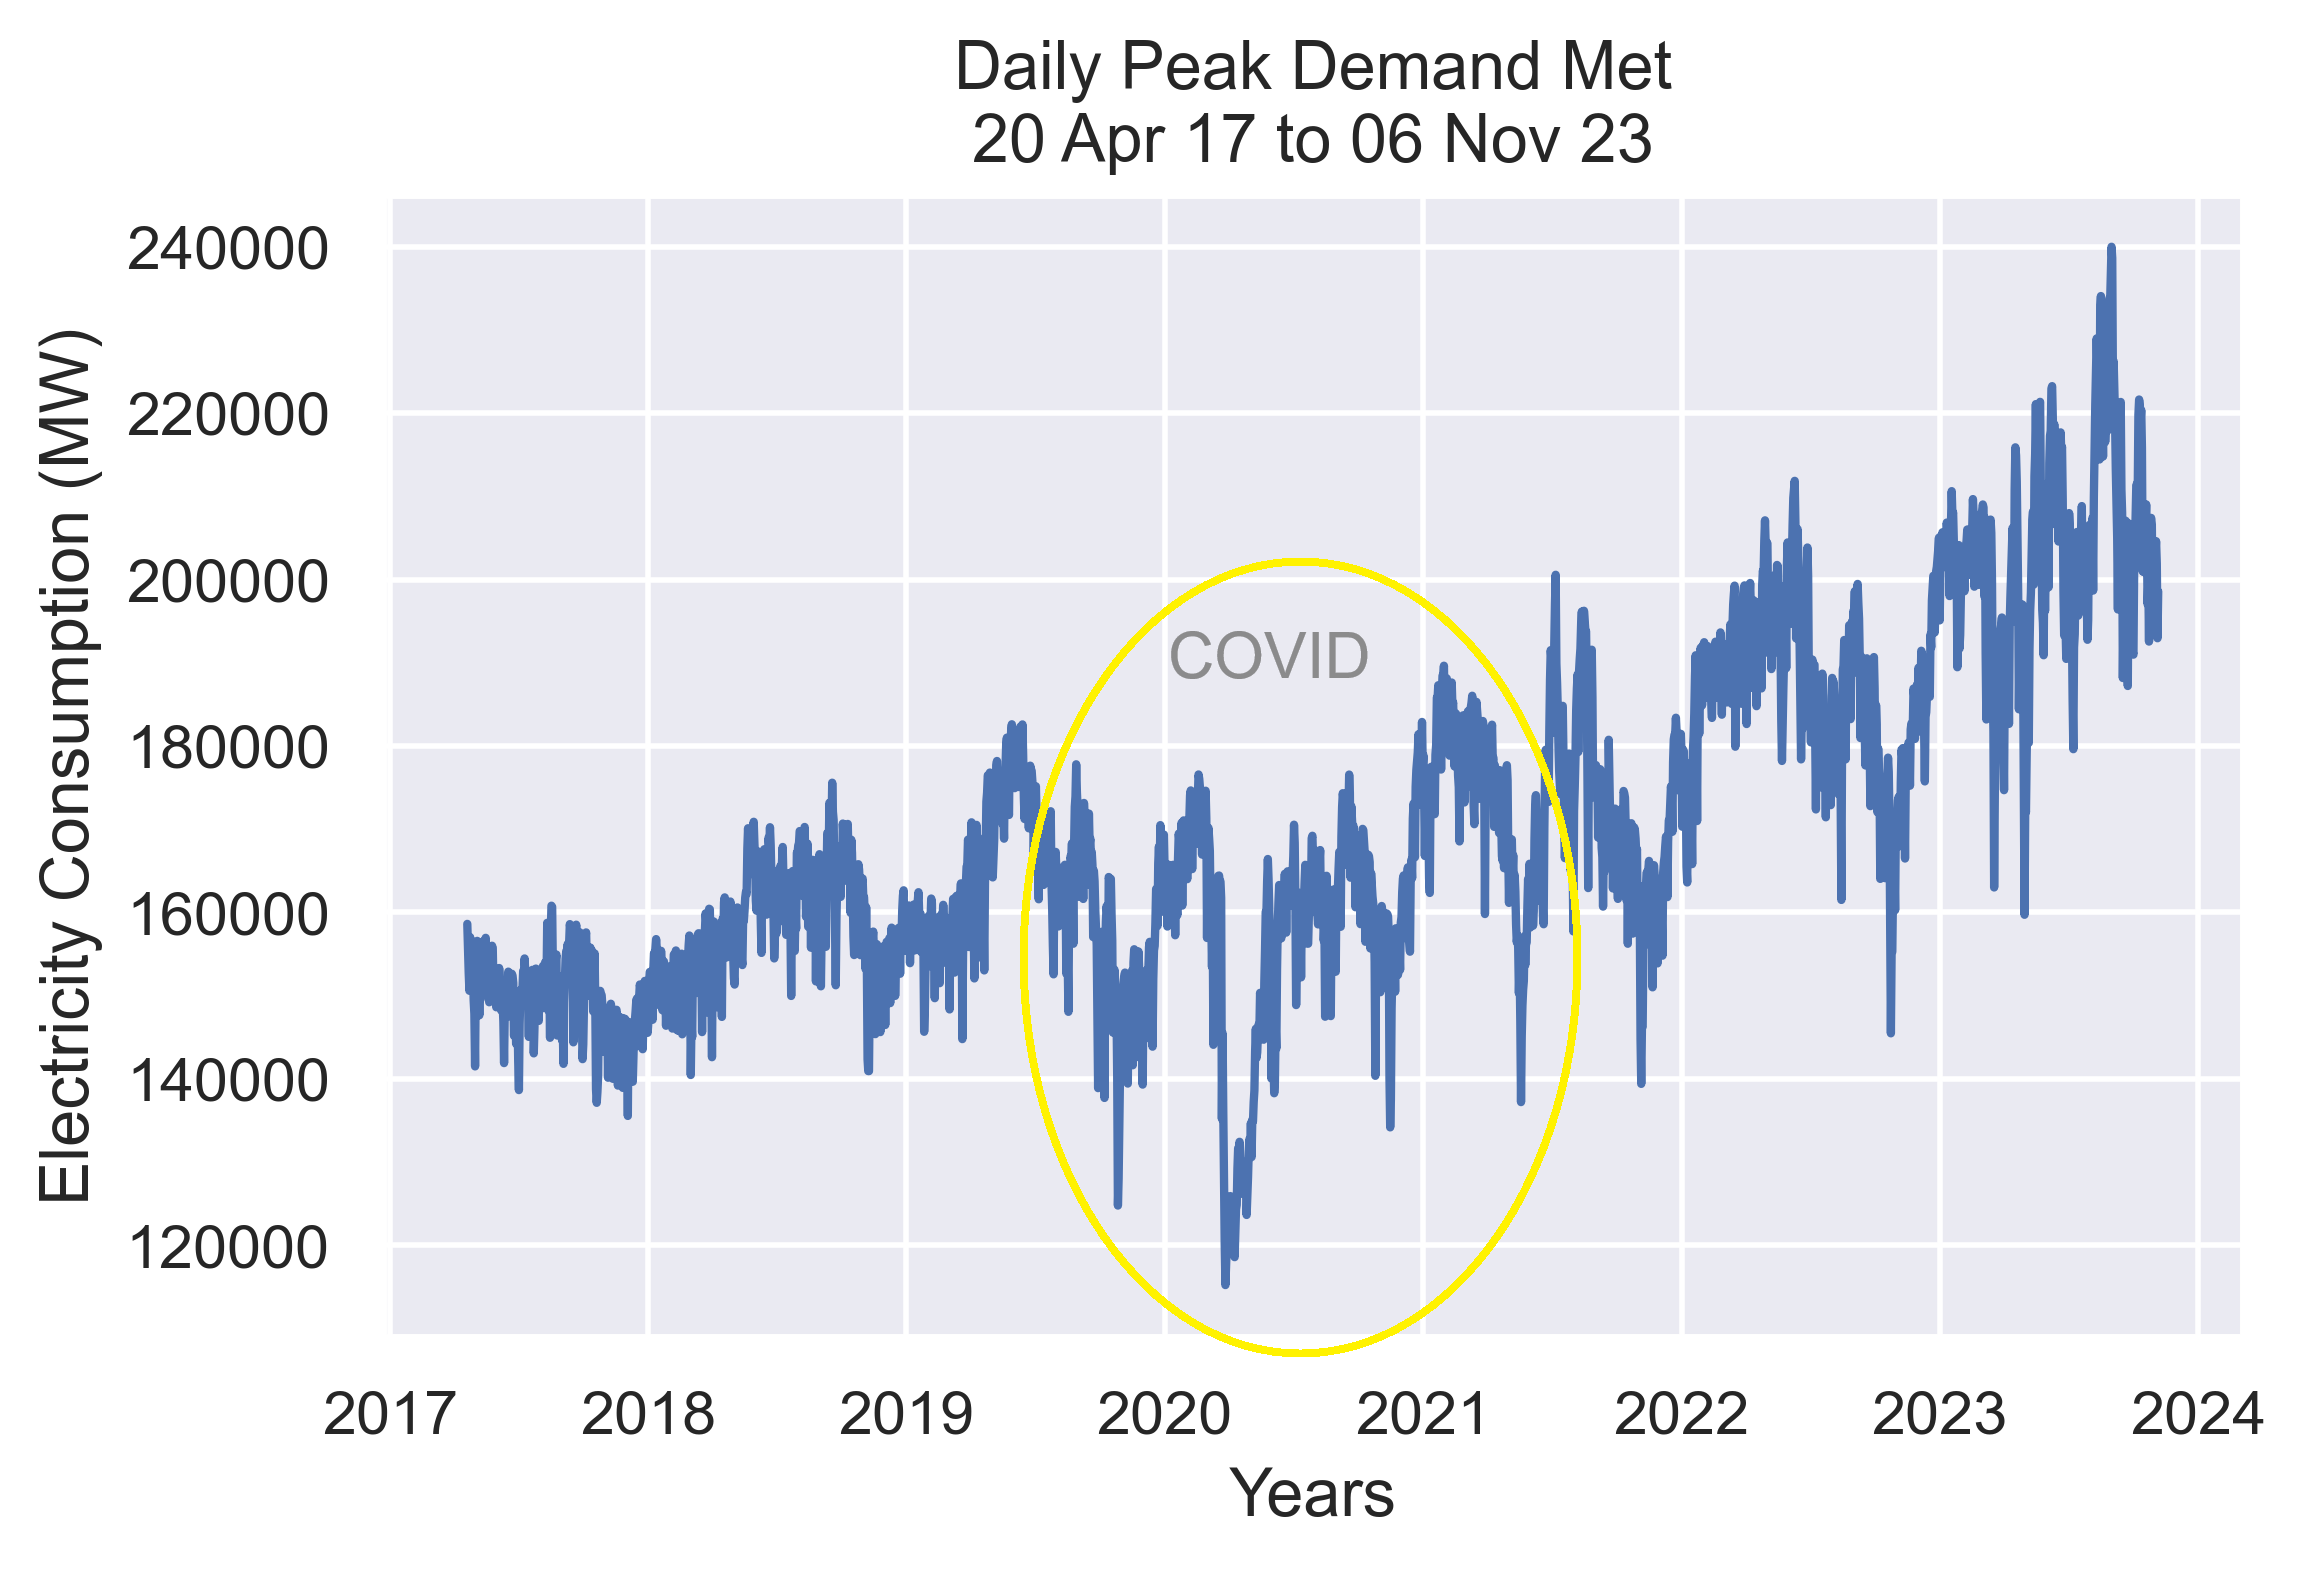
\includegraphics[scale=.75]{images/Daily Peak1.png}
\credit{https://iced.niti.gov.in/}
\end{frame}
\note[itemize]{
\item Data from niti ayog website
\item From Apr 17 to Nov 23
\item Effect of Covid
\item Lets Decompose the time series
}
\subsection{Decomposition}
\begin{frame}{Time series-Decomposed (Yearly Seasonality) }
\centering
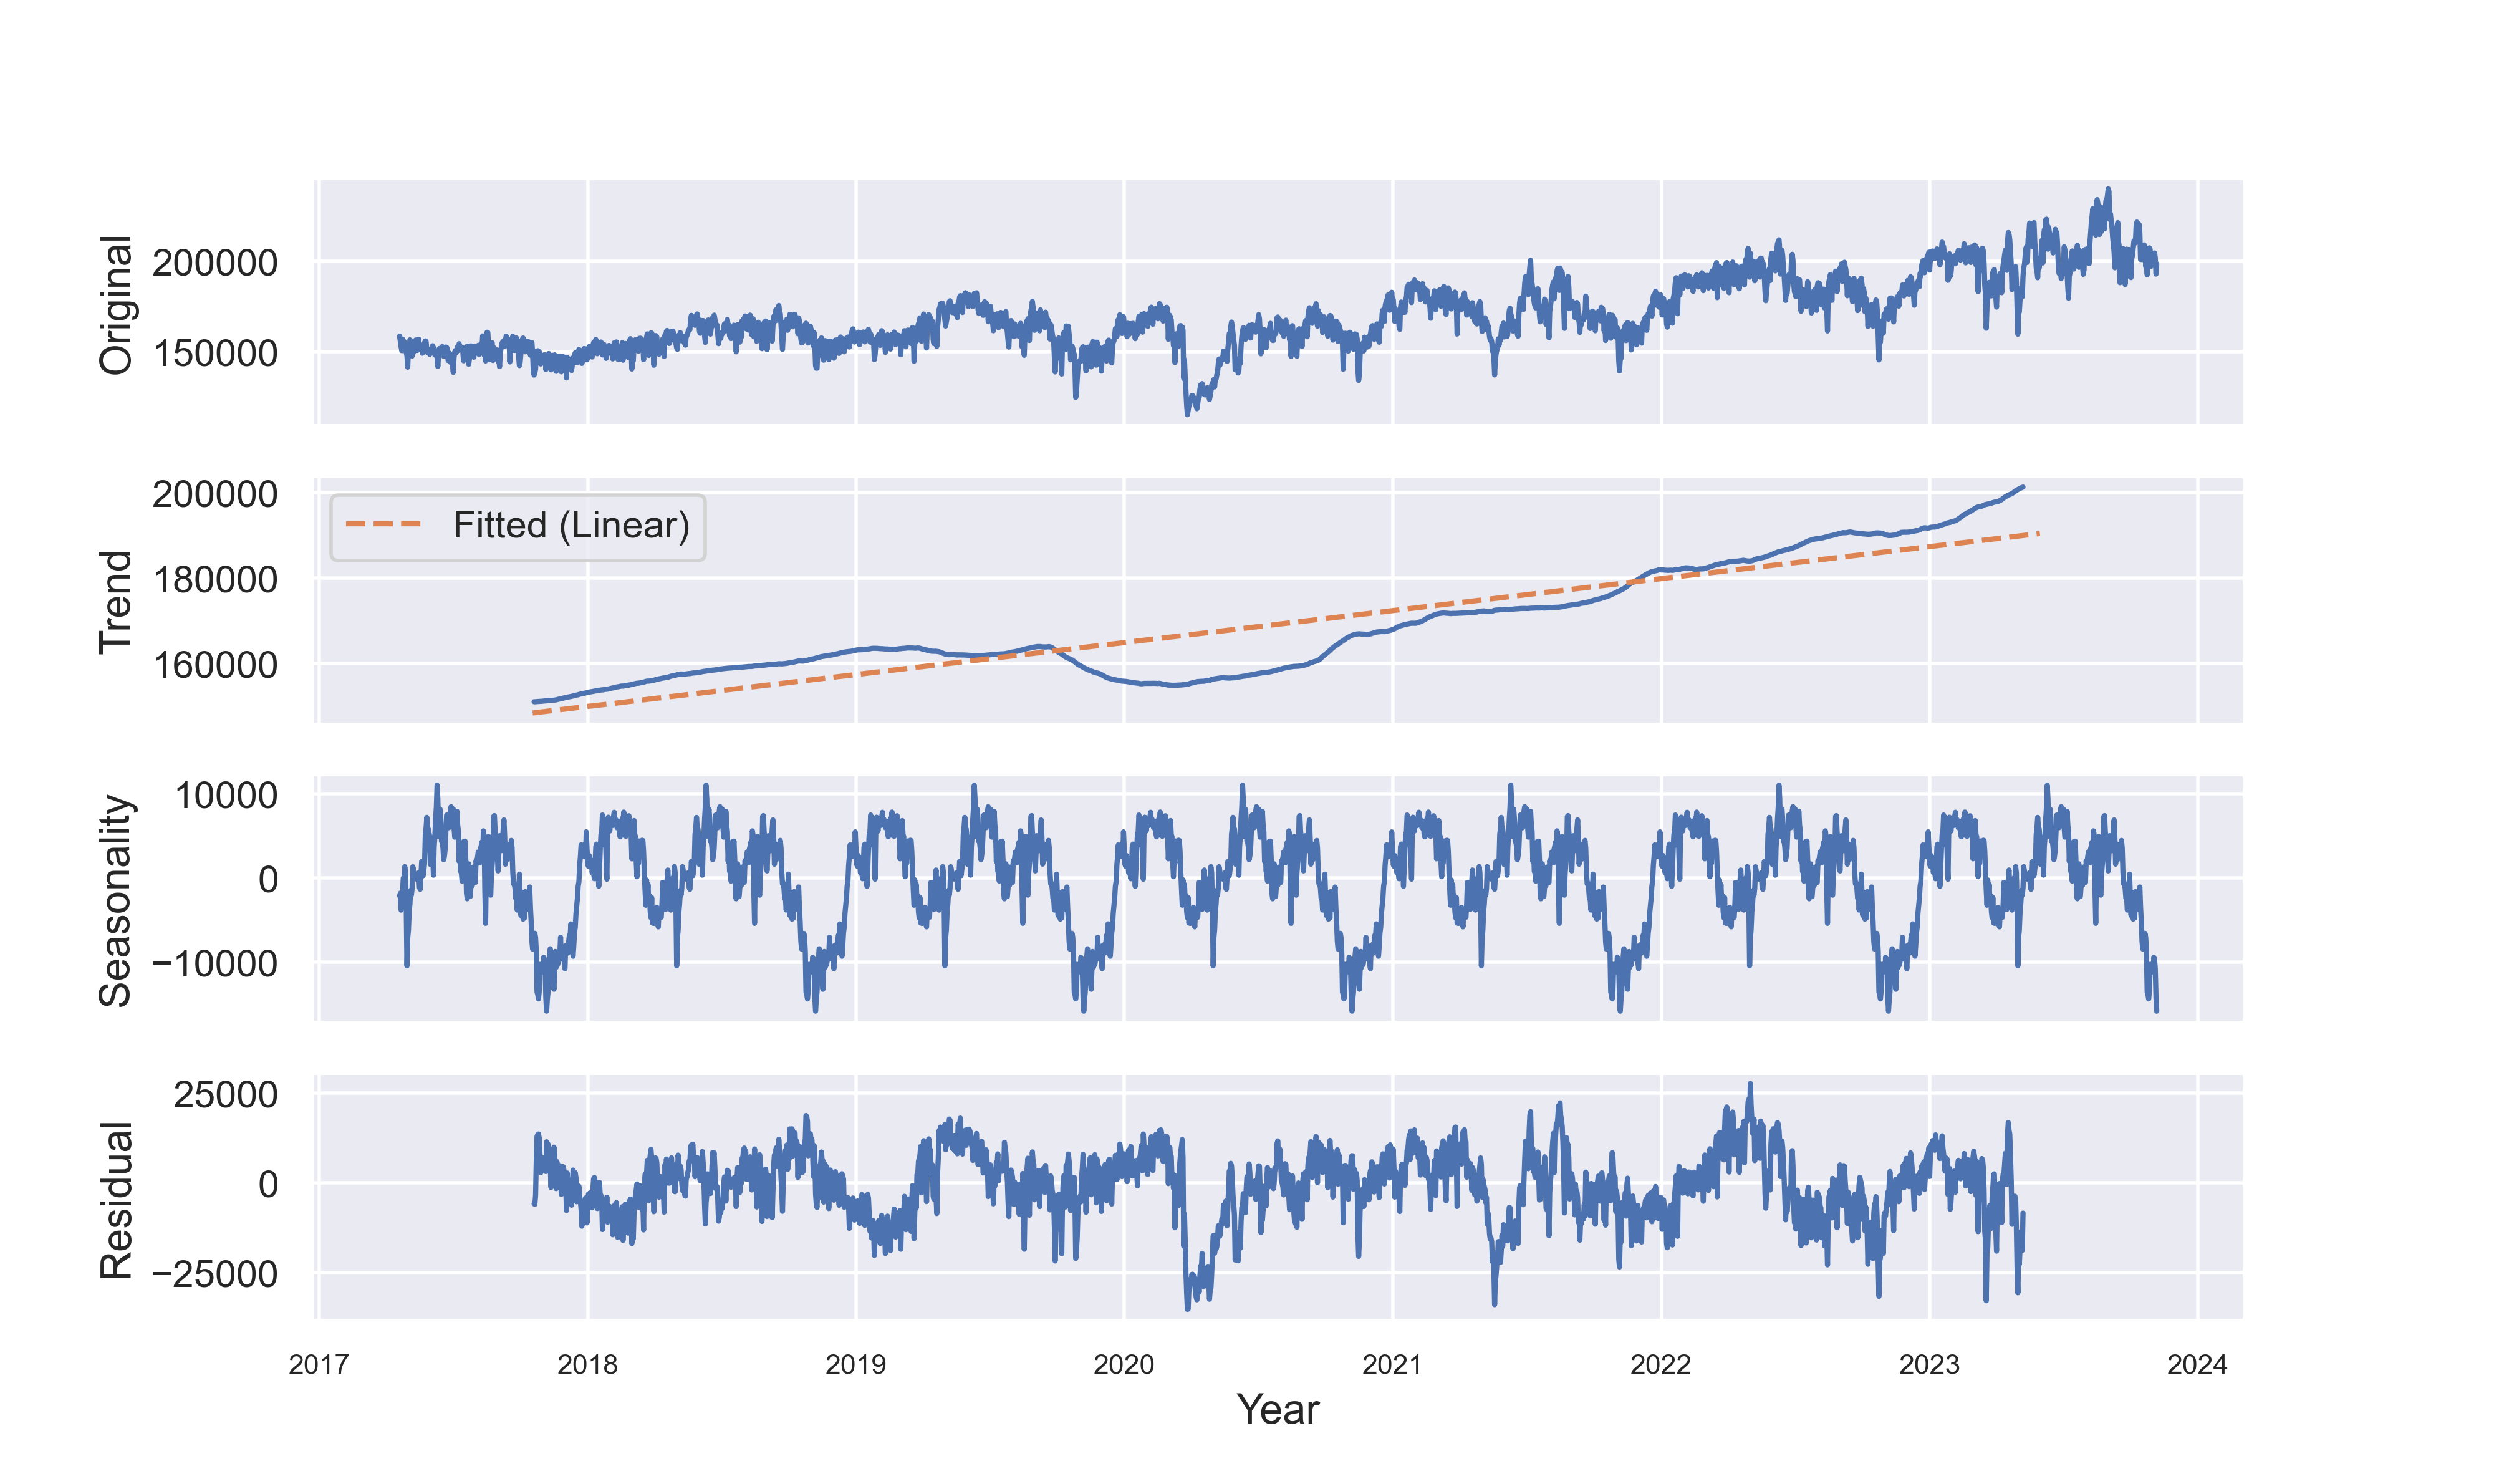
\includegraphics[scale=.50]{images/Decompose.png}
\credit{https://iced.niti.gov.in/}
\end{frame}
\note[itemize]{
\item Trend seems to be linear
\item Have Yearly Seasonality
\item Effect of Covid
\item Lets Decompose the time series
}
\subsection{Trend and Seasonality}
\begin{frame}{Train/Test- Linear Trend with Yearly Seasonality\\(Ordinary Least Square) }
\centering
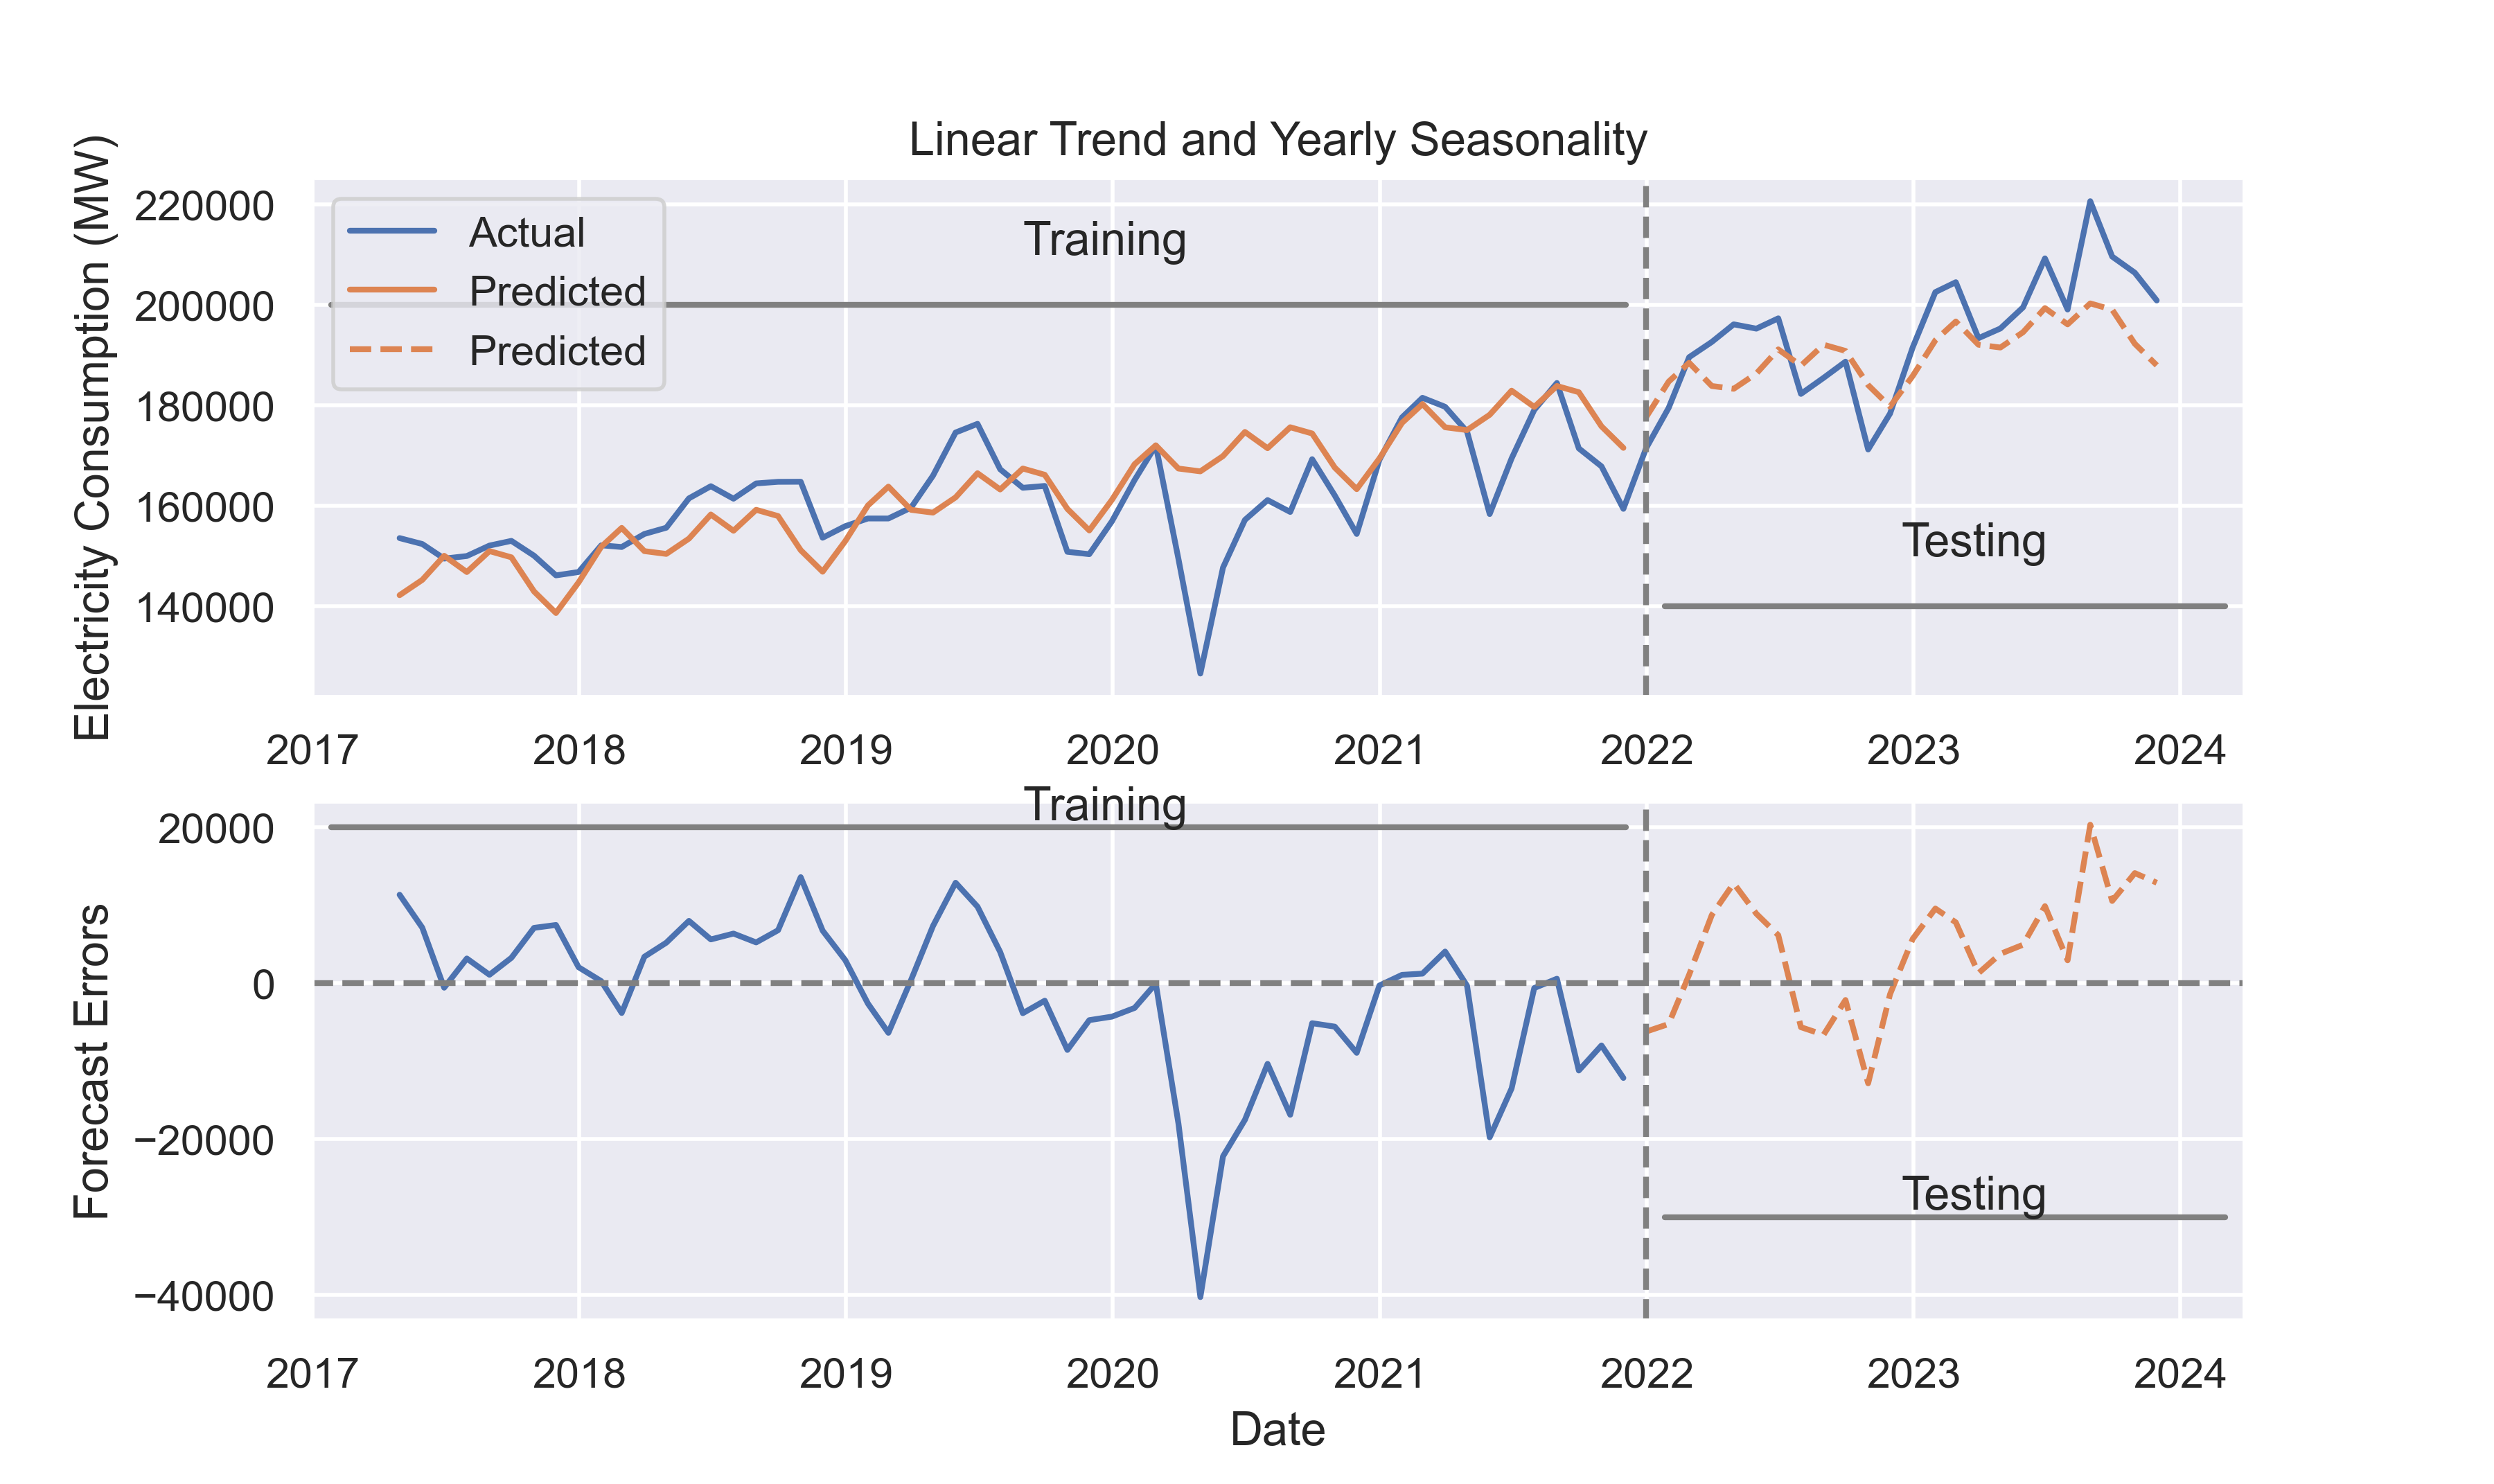
\includegraphics[width=\linewidth]{images/Monthly_test_train.png}
\credit{https://iced.niti.gov.in/}

\end{frame}
\note[itemize]{
\item Trend seems to be linear
\item Have Yearly Seasonality
\item Effect of Covid

}


\begin{frame}{Train/Test- Linear Trend with Yearly Seasonality \\Error Metrics  }
\centering
\begin{columns}[t]
 \begin{column}{0.48\textwidth}
 
  \begin{block}{}
   \begin{figure}
    \centering
        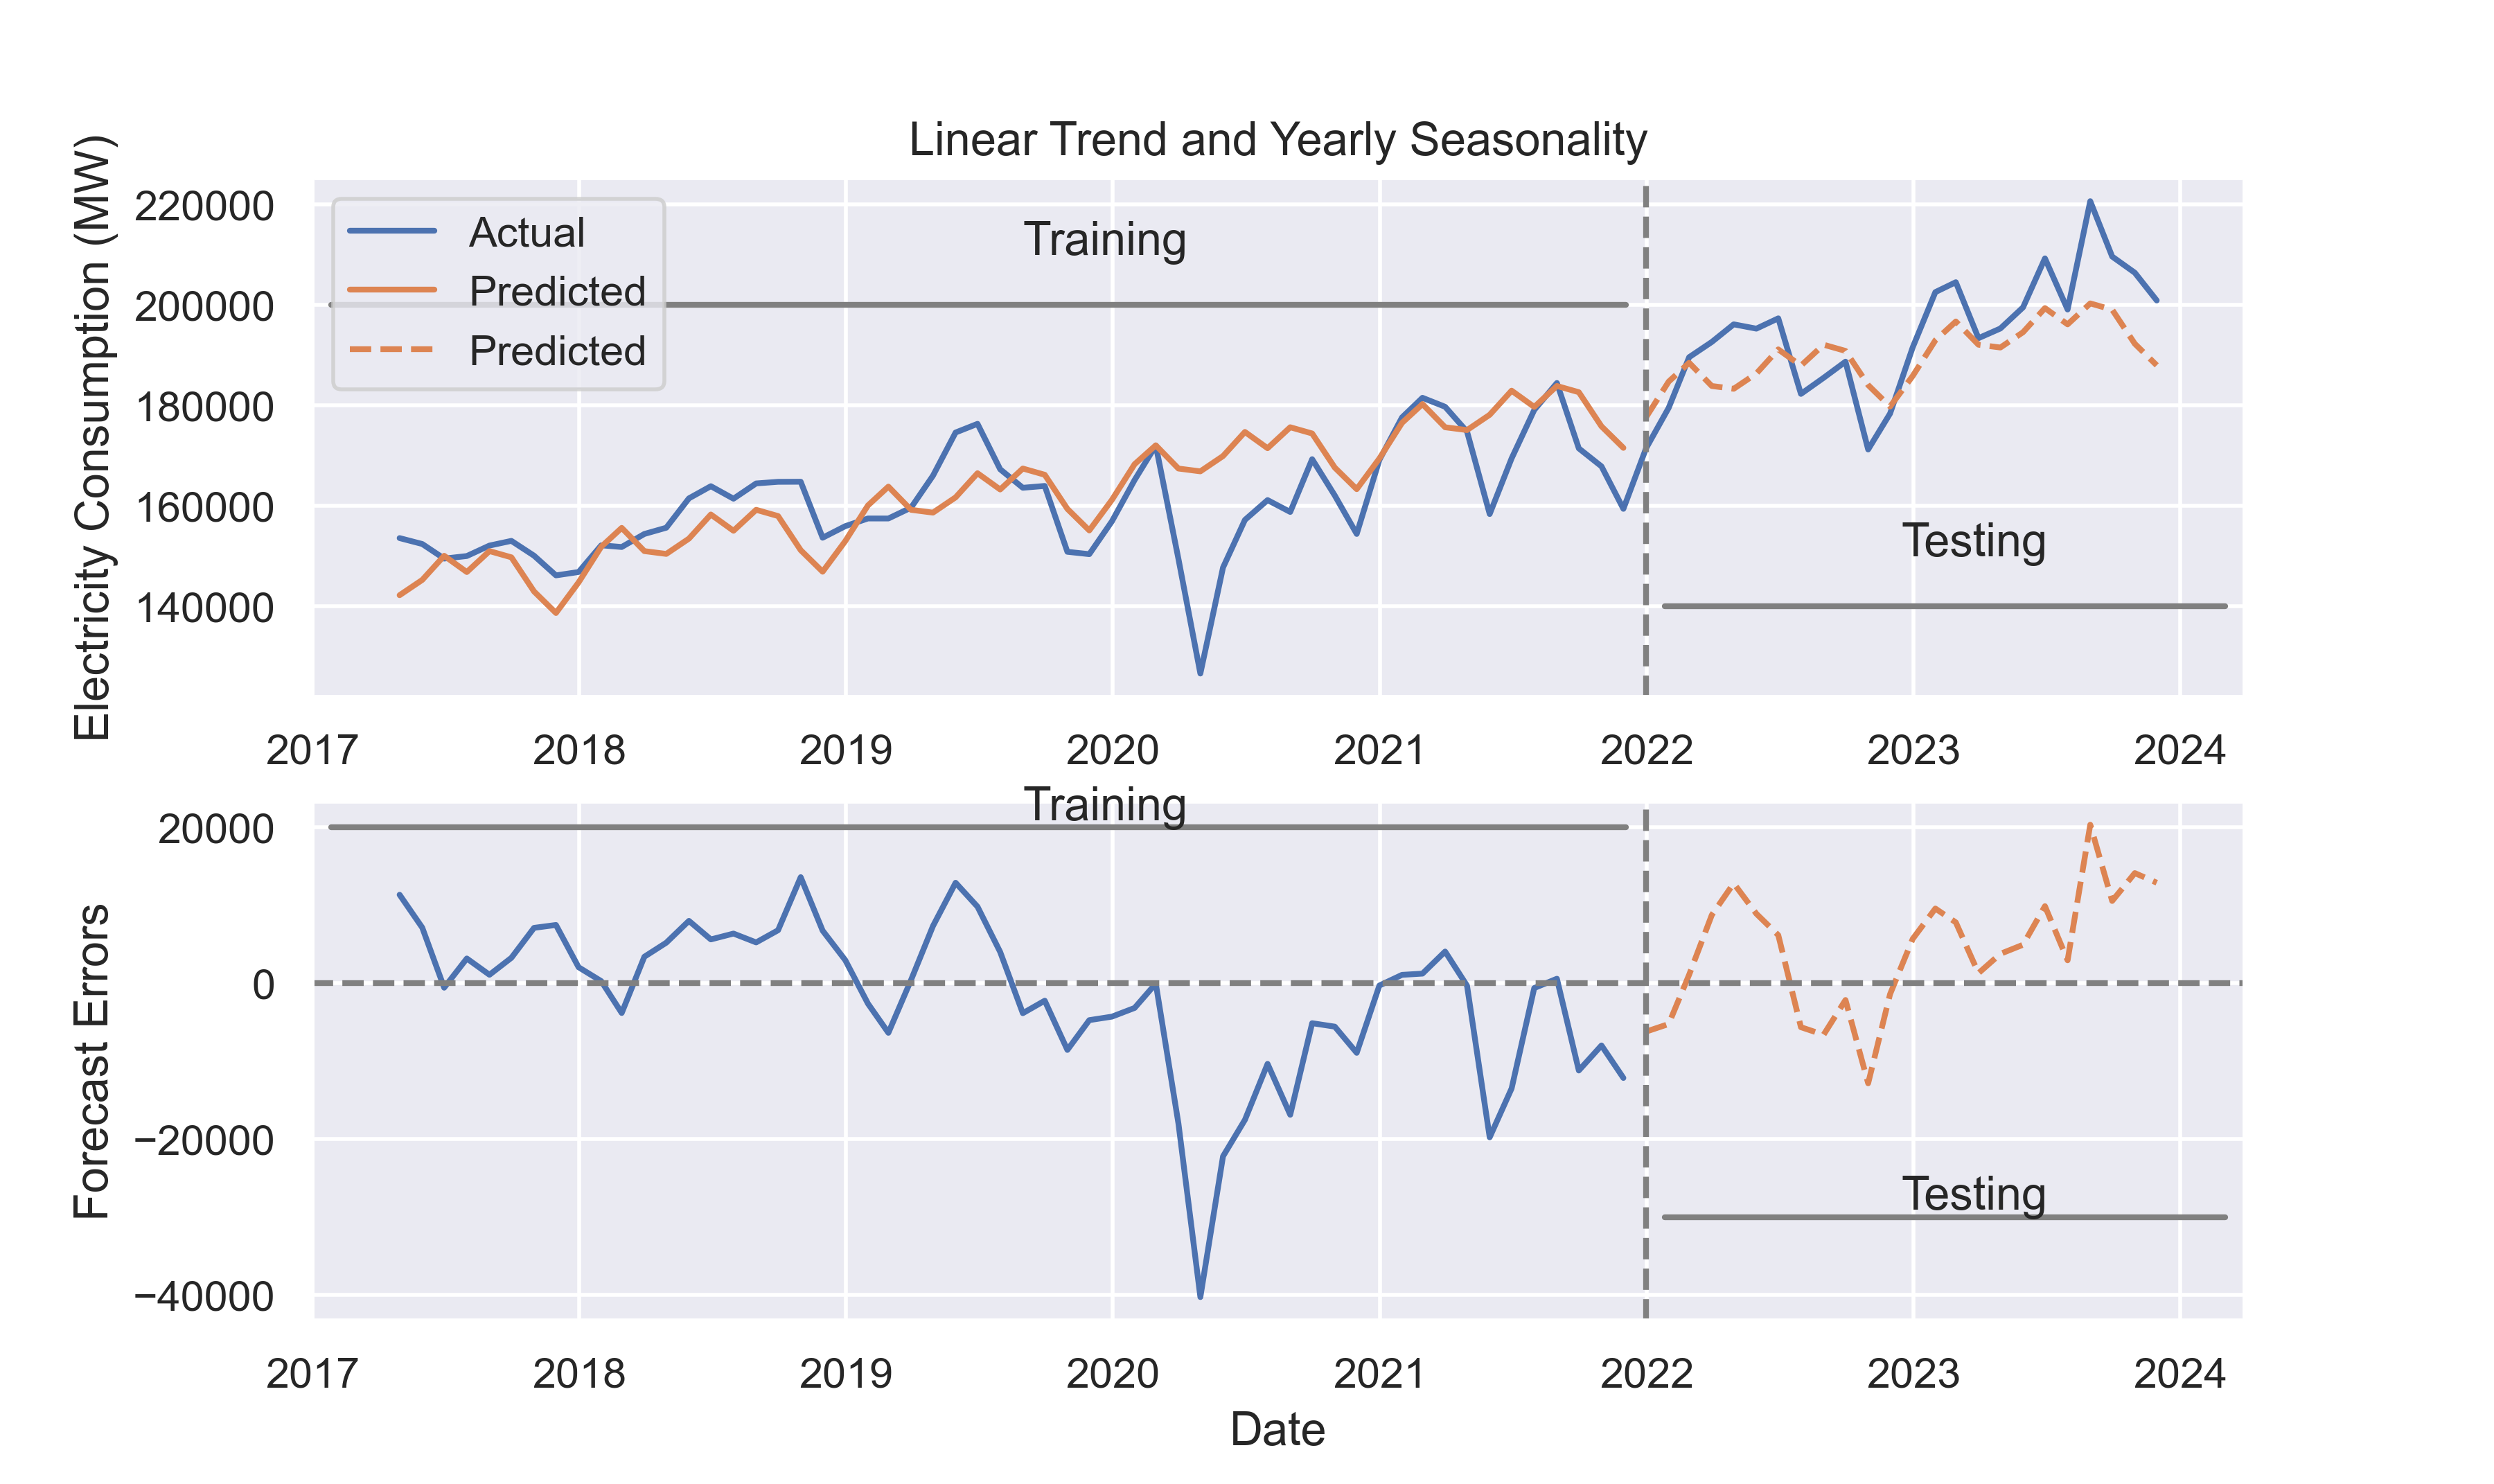
\includegraphics[width=\linewidth]{images/Monthly_test_train.png}
        \label{fig:a}
   \end{figure}
  \end{block}   
 \end{column}
 \begin{column}{0.48\textwidth}
 
  \begin{block}{Error Metrics}
   
    \centering
       \begin{tabular}{l|r|r}
\toprule
 & \multicolumn{2}{c}{OLS} \\
Measure & Test & Train \\
\midrule
MAE & 7129.32 & 7576.00 \\
\midrule
MAPE & 0.05 & 0.04 \\
\midrule
RMSE & 9948.14 & 8894.58\\
\bottomrule
\end{tabular}
   
  \end{block}   
 \end{column}

\end{columns}
\end{frame}
\note[itemize]{
\item Trend seems to be linear
\item Have Yearly Seasonality
\item Effect of Covid
\item Lets Analyse Autocorrelation between neighbouring values
}

\subsection{Smoothing - Holts Winters }
\begin{frame}{Holt Winters}
\centering
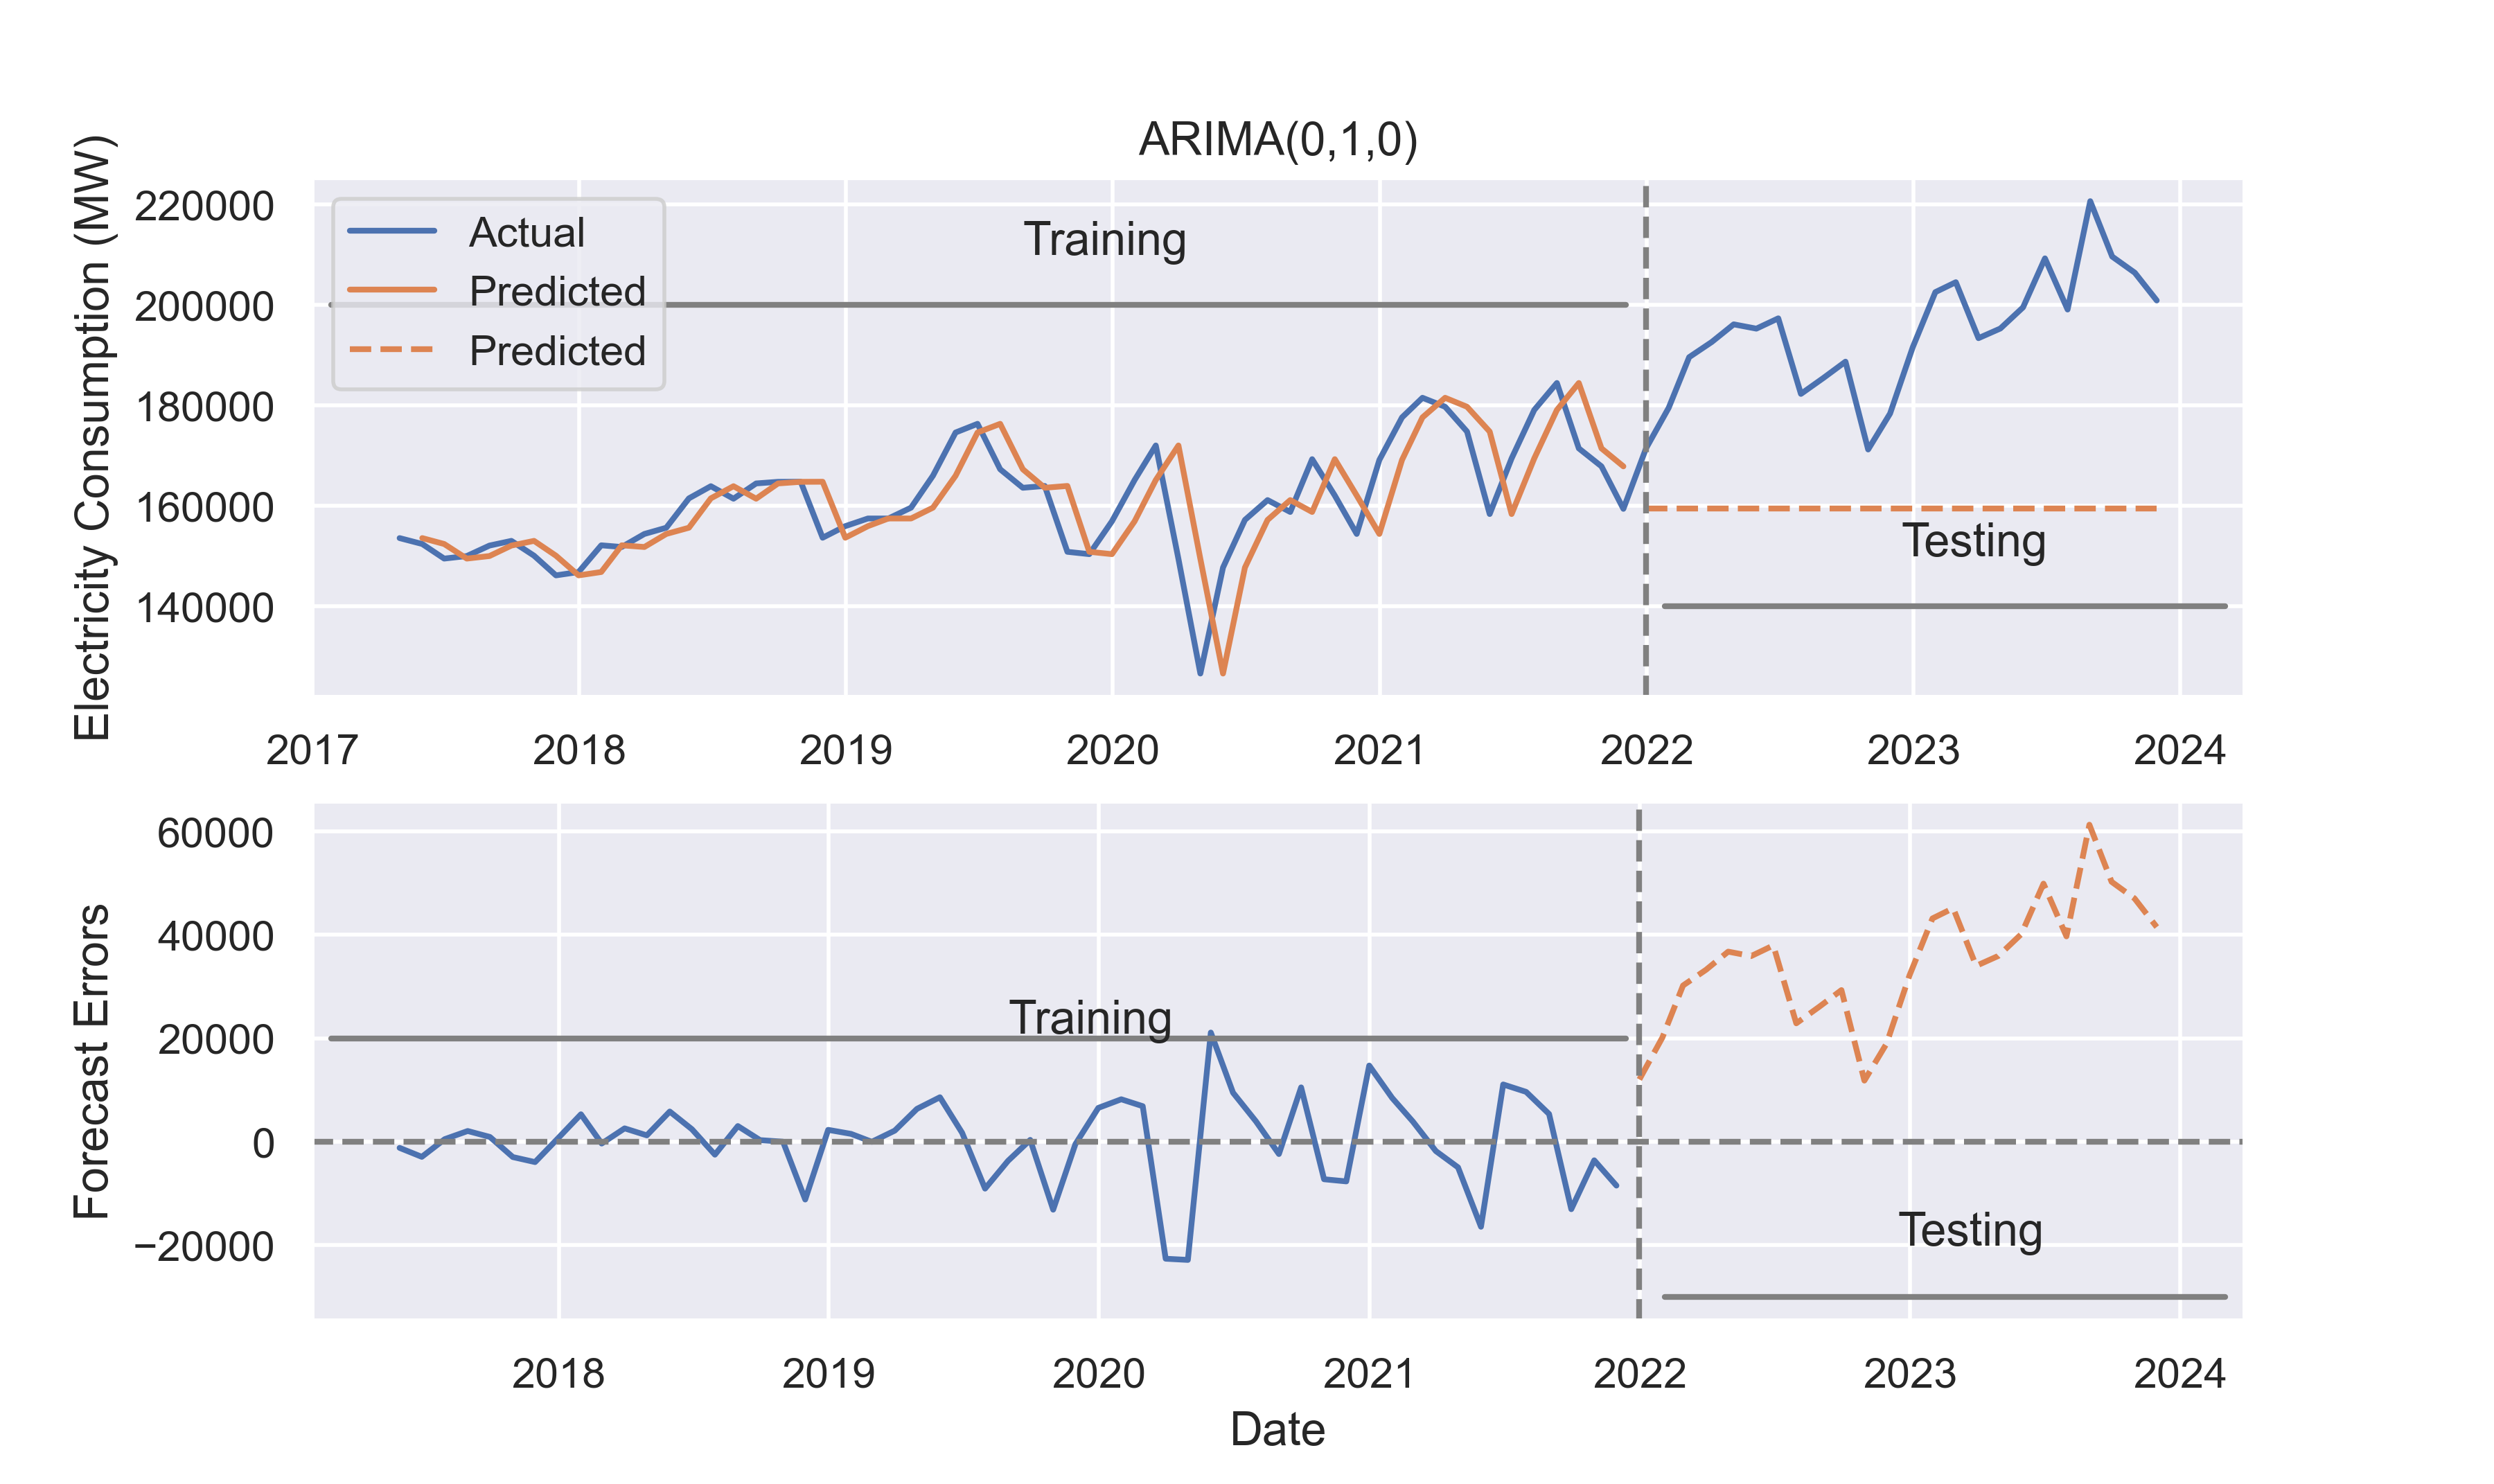
\includegraphics[width=\linewidth]{images/Holt Winters.png}
\credit{https://iced.niti.gov.in/}
\end{frame}
\note[itemize]{
\item Trend seems to be linear

}

\begin{frame}{Error Metrics - OLS vs Holt Winters }
\centering
 
  \begin{block}{Error Metrics}
   
    \centering
       \begin{tabular}{l|l|l|l|l}
\toprule
 Measure & \multicolumn{2}{c}{OLS}  & \multicolumn{2}{c}{HW} \\
 
 \midrule
 & Test & Train &Test&Train\\
\midrule
MAE & 7129.32 & 7576.00 &5815.48&16401.85\\
\midrule
MAPE & 0.05 & 0.04 &0.040 & 0.08\\
\midrule
RMSE & 9948.14 & 8894.58& 7801.94 & 18157.35 \\
\bottomrule
\end{tabular}
   
  \end{block}
\end{frame}

\subsection{Auto correlation and auto regressive models}
\begin{frame}{Autocorrelation-PACF of Series and Residual}
\centering
\includegraphics[width=\linewidth]{images/Pacf_both.png}
\credit{https://iced.niti.gov.in/}
\end{frame}
\note[itemize]{
\item Trend seems to be linear

}

\begin{frame}{Daily Load Curve}
\centering
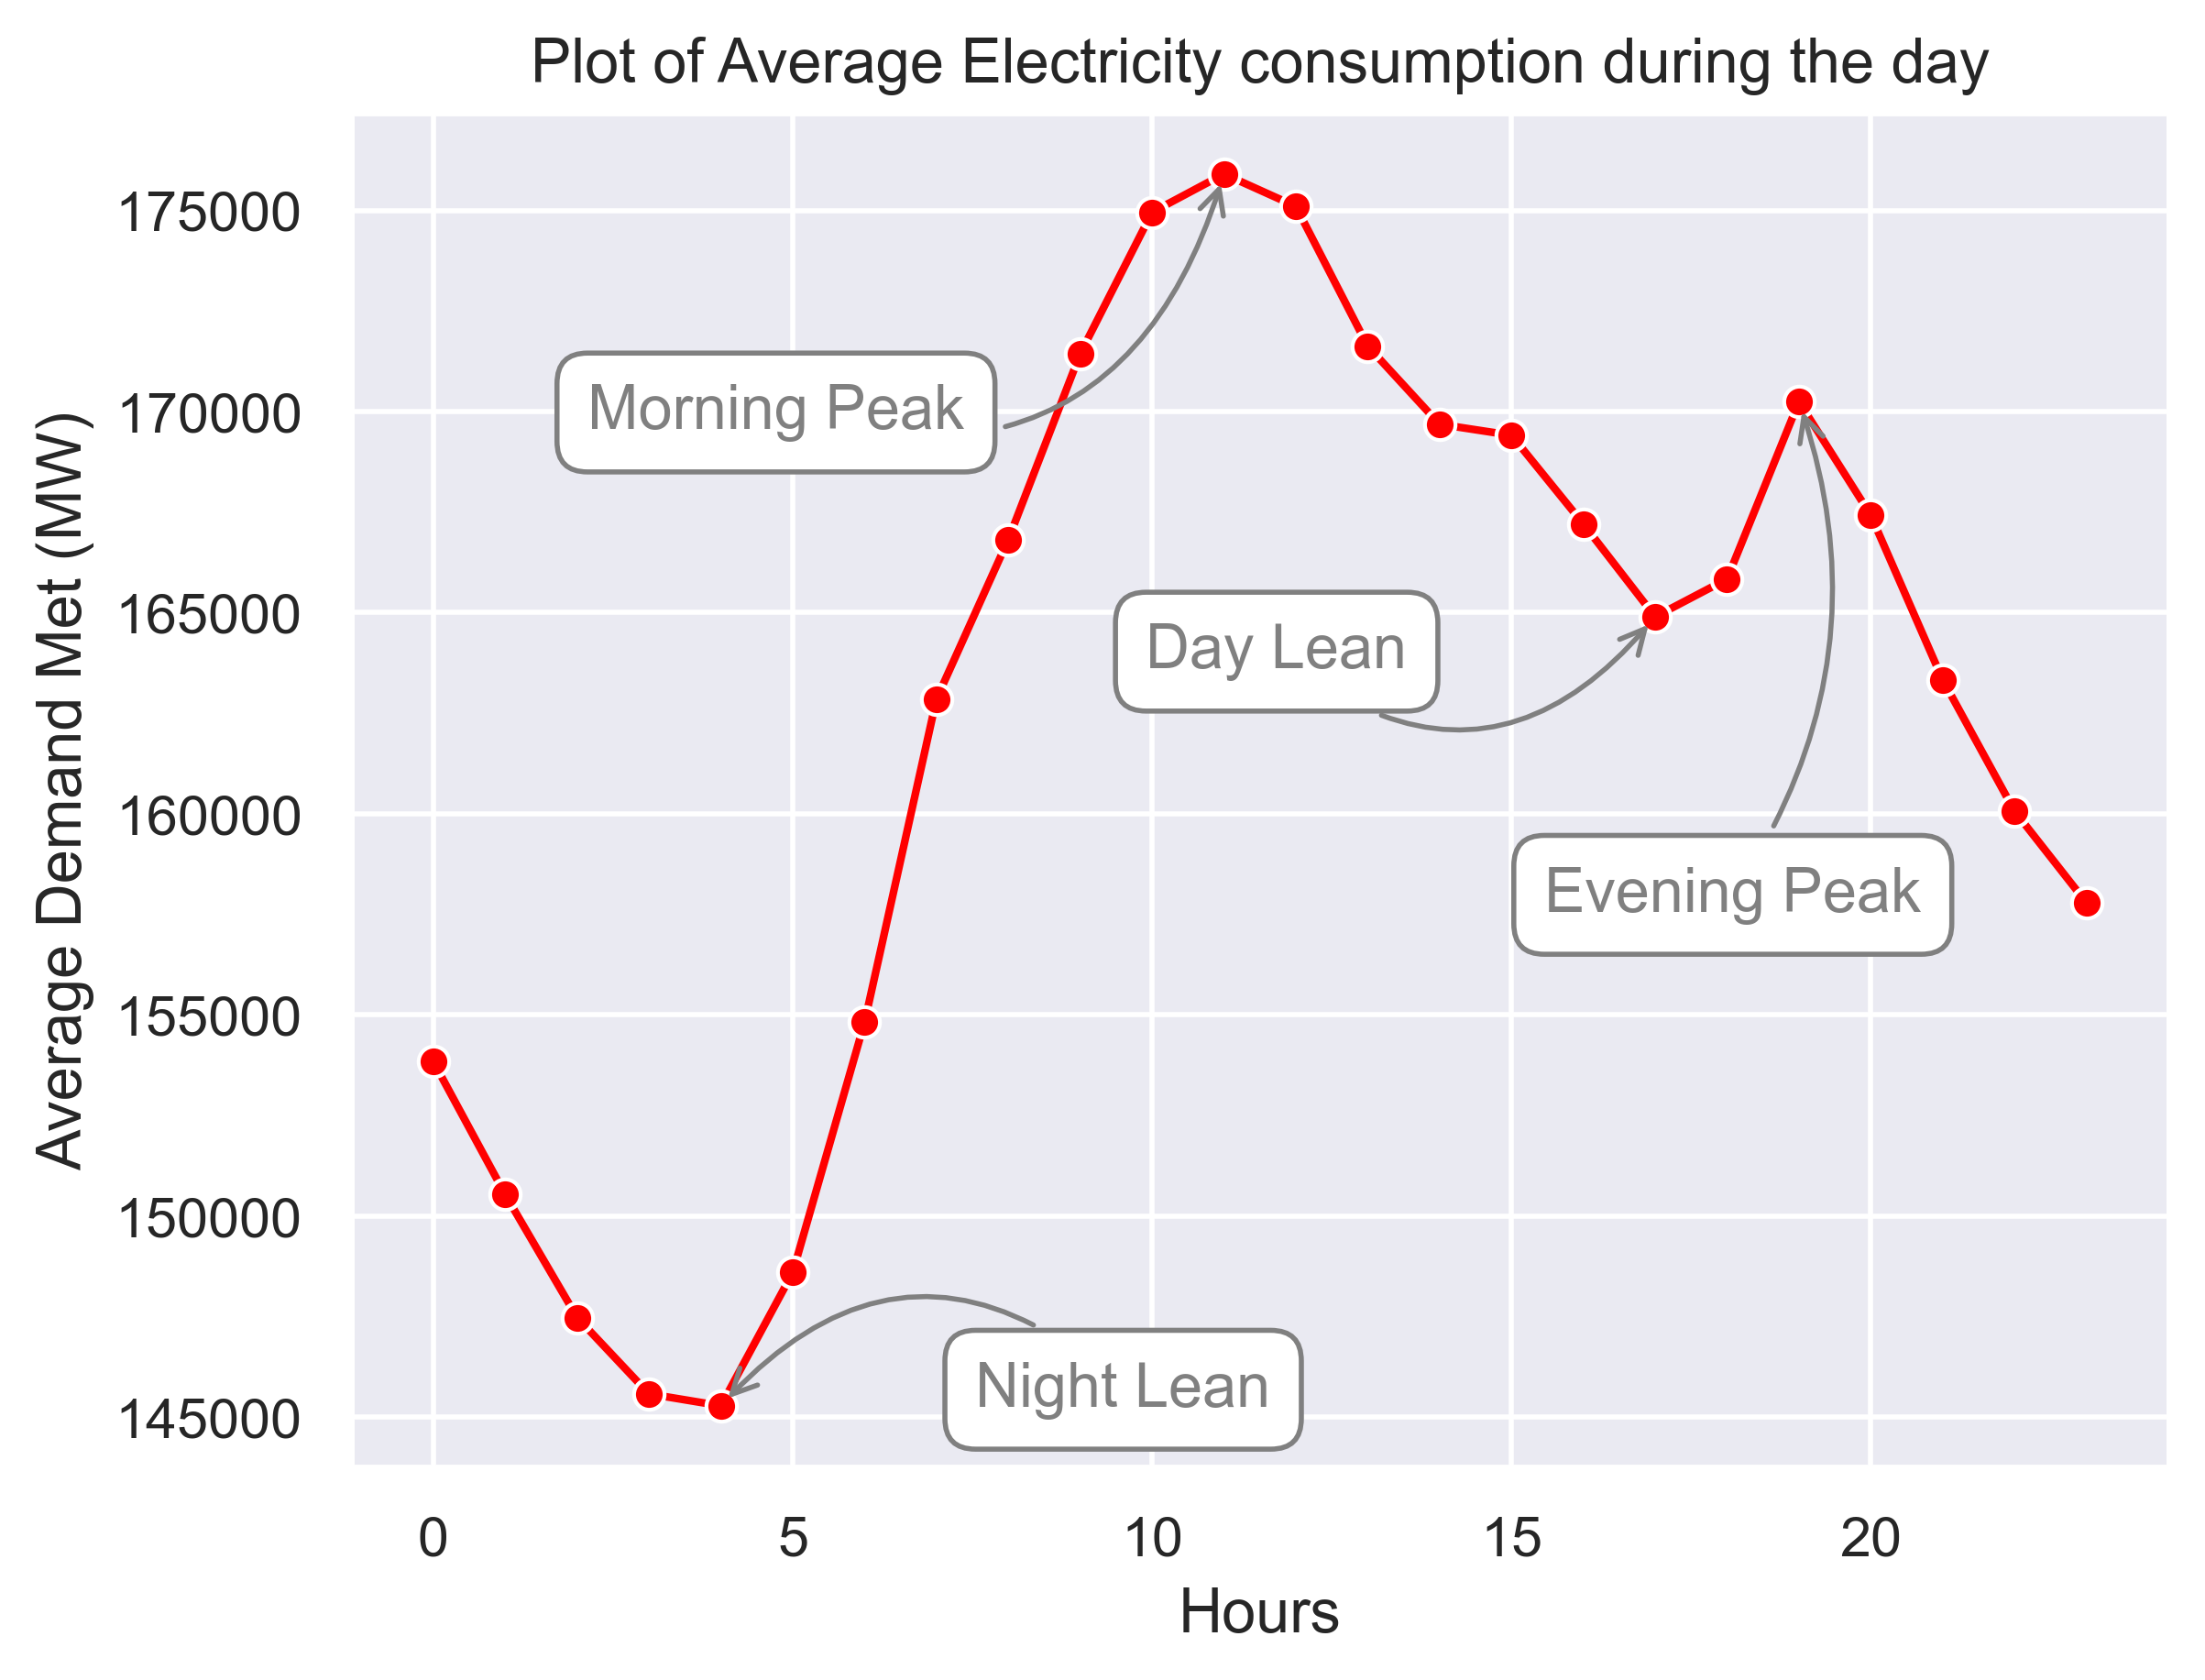
\includegraphics[scale=.60]{images/Load Curve.png}
\credit{https://iced.niti.gov.in/}
\end{frame}

\begin{frame}{Consumption - Consumer Wise}
\centering
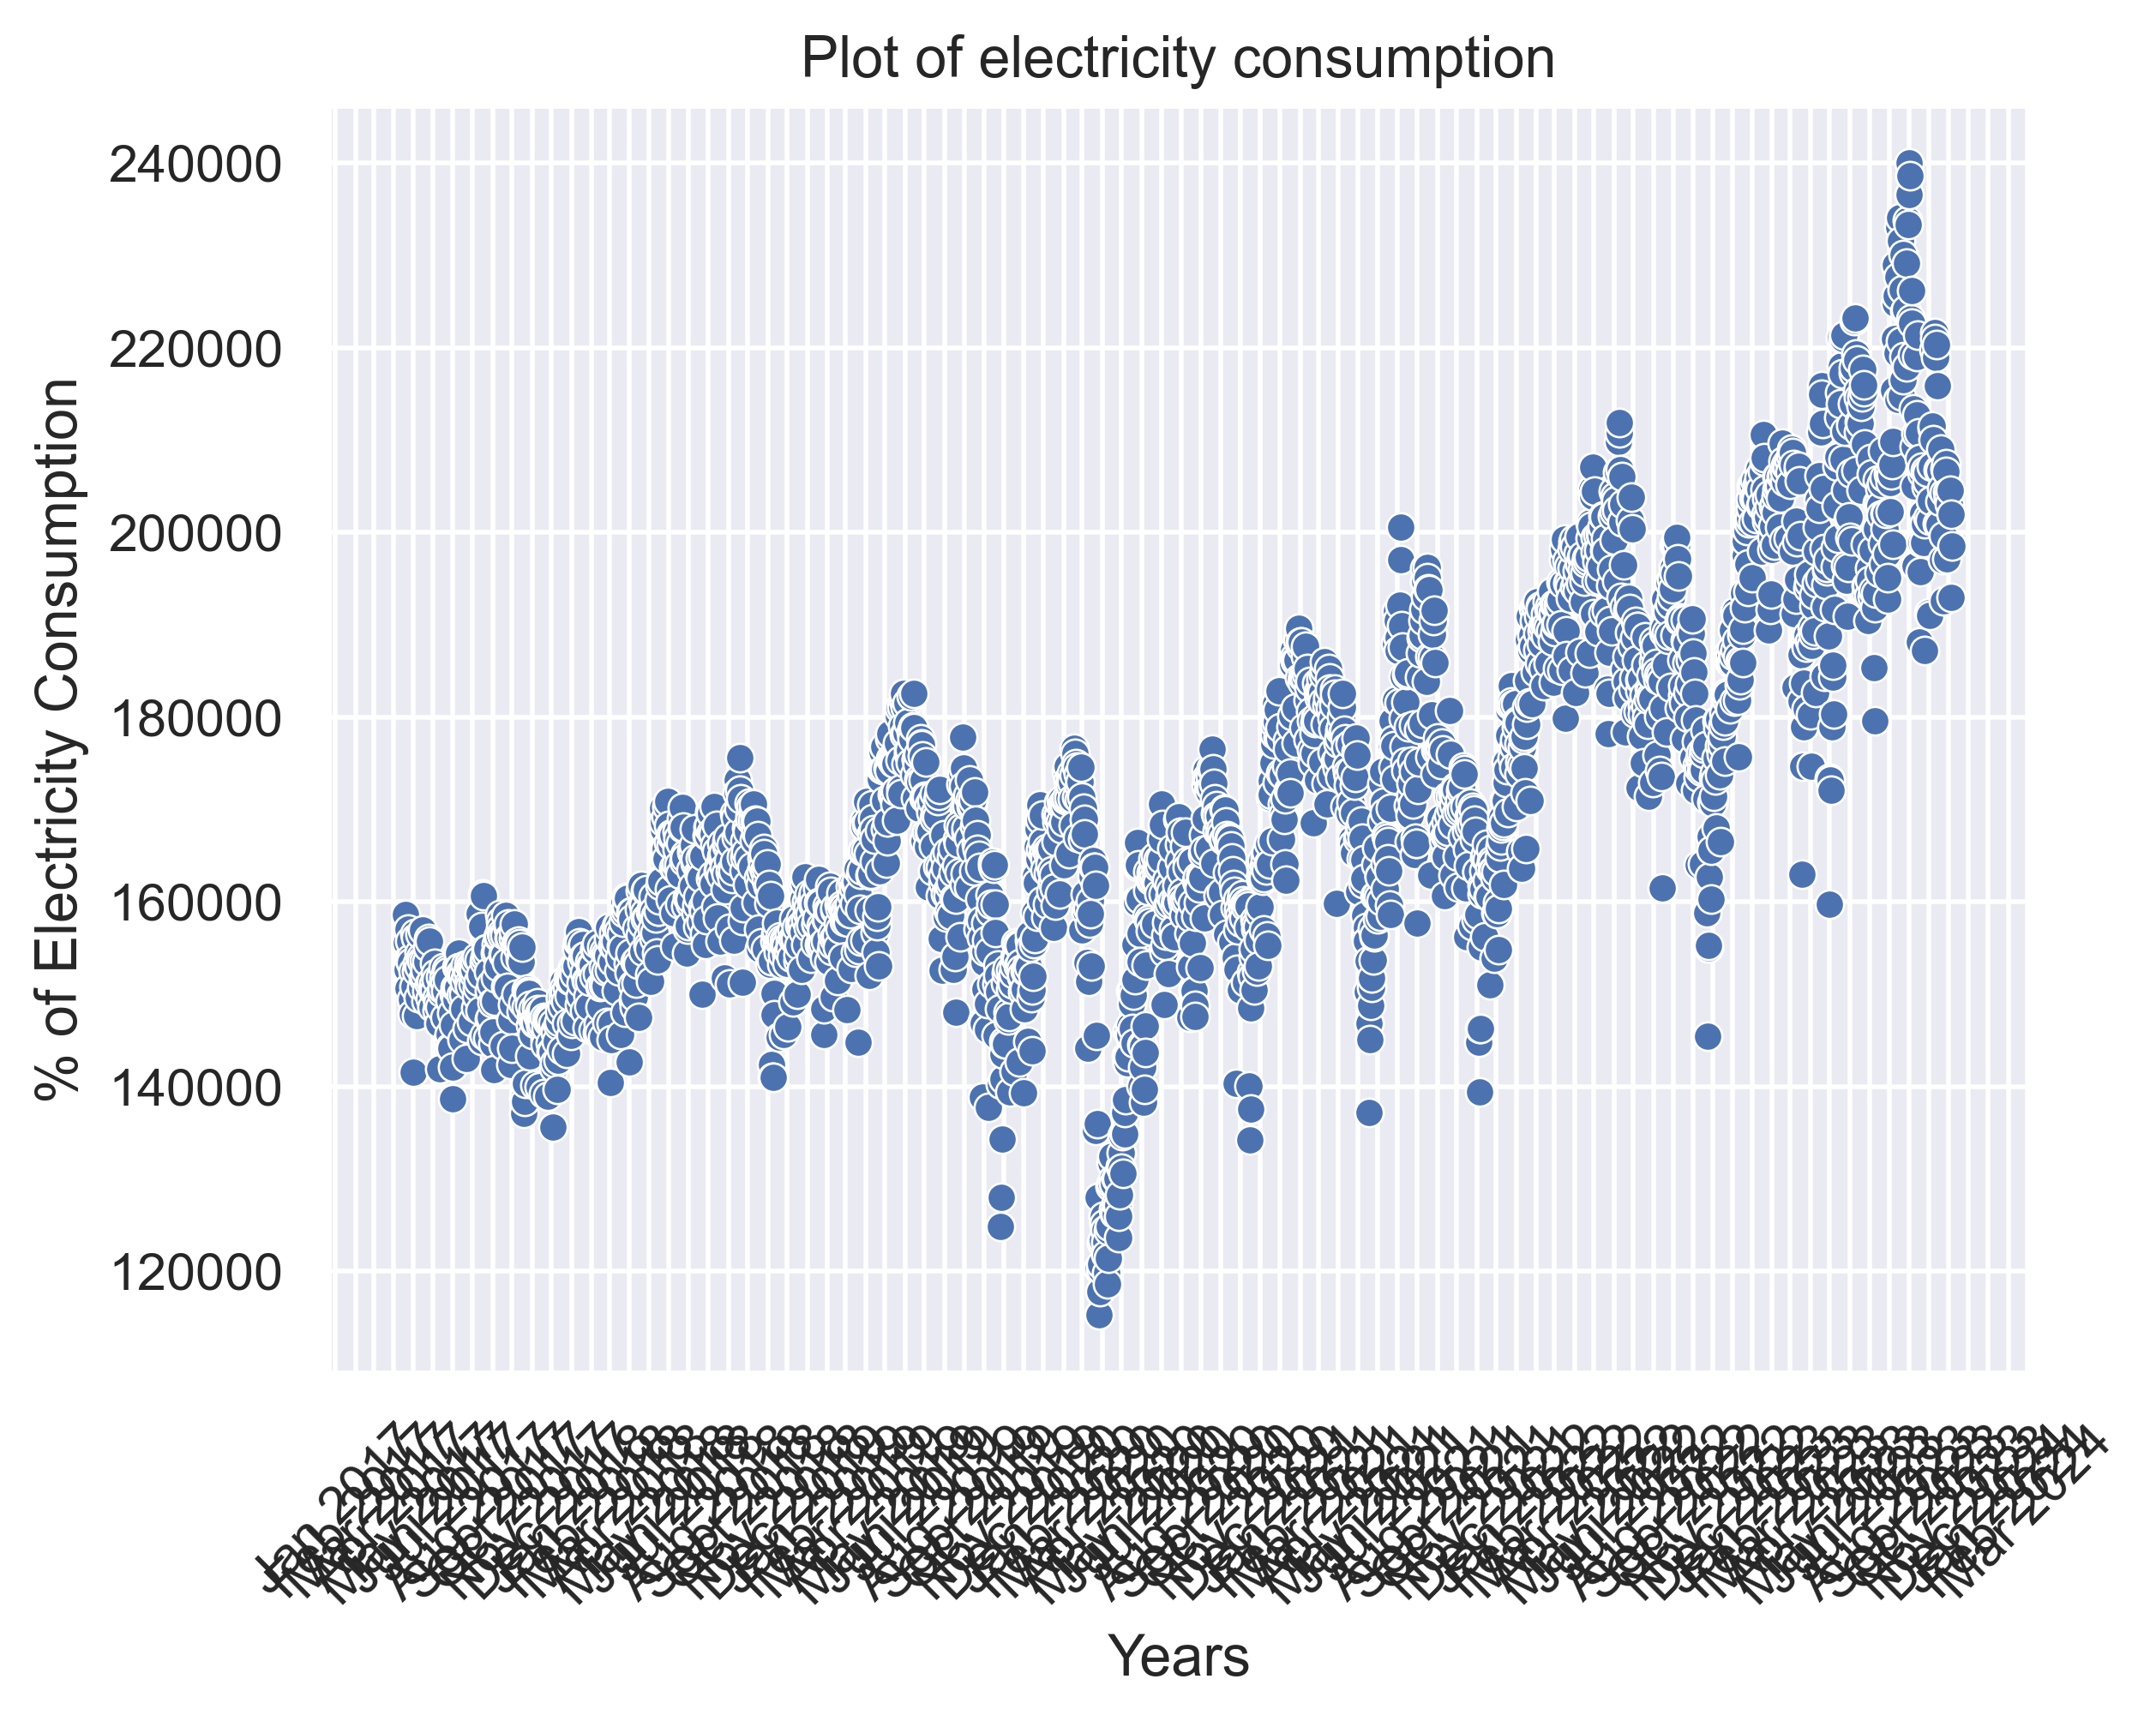
\includegraphics[scale=.55]{images/Cons_Ind_wise.png}
\credit{https://cea.nic.in/}
\end{frame}

\end{document}